\section{مقدمه}

در این پروژه قصد داریم بدافزار میرای (\lr{Mirai}) را شیبه‌سازی کنیم. میرای با دسترسی به تعداد کثیری از سیستم‌ها و ارسال درخواست \lr{DNS}، \lr{Dyn} سرورها را از کار می‌انداخت و باعث قطع دسترسی بسیاری از وبسایت‌های معروف دنیا می‌شد. 

هدف این پروژه ساخت برنامه‌ای است که پورت‌های باز موجود در شبکه که \lr{ssh} در آن‌ها اجرا می‌شود را پیدا کند و سپس با تست کردن رمز عبور‌های معروف که در تعداد زیادی از دستگاه‌ها استفاده می‌شوند به این سیستم‌ها دسترسی پیداکرده و با پیاده‌سازی یک بدافزار روی آن‌ها اطلاعات امنیتی این سیستم‌ها را به یک سرور مشخص ارسال کند. 

\section{ساختار شبکه}

در این پروژه با استفاده از داکر یک شبکه ایجاد کرده و تعدادی کانتینر به آن اضافه کرده و درنهایت یک حمله را در این شبکه شبیه سازی کرده‌ایم.  

این شبکه دارای سه نوع \lr{image} است: وب‌سرور، حمله‌کننده و سرور هدف. برای هر \lr{image} یک \lr{Dockerfile} پیاده‌شده که از \lr{image}های سرورهدف چند و از \lr{image}های سیستم‌های وب‌سرور و حمله‌کننده تنها یک کانتینر ایجاد می‌شوند. 

\section{وب‌سرور}

از این وب سرور که با جنگو پیاده سازی‌شده برای اهداف مختلفی مانند ارسال اطلاعات امنیتی جمع آوری شده از سیستم‌های مورد حمله قرار گرفته و ارسال به این سرور و ذخیره اطلاعات در این دیتابیس و دانلود بدافزار توسط سیستم های قربانی از این سرور استفاده می‌شود. 

اسکریپت \lr{infocrawler.sh} در این وب سرور ذخیره‌شده‌است که روی سیستم مورد هدف دانلود شده و اطلاعات امنیتی سیستم هدف را به صورت \lr{json} به وب‌سرور ارسال میکند. 

\begin{figure}[h!]
    \centering
    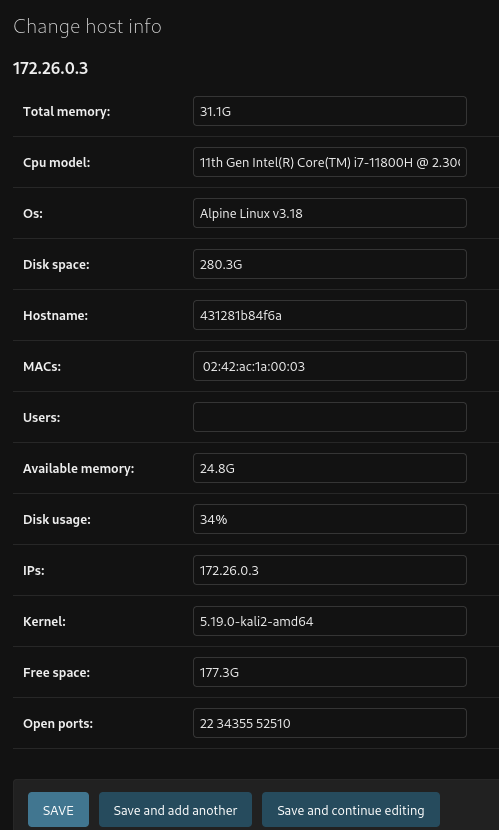
\includegraphics[width=0.5\linewidth]{images/sample_host.png}
    \caption{نمونه اطلاعات استخراج شده از سیستم هدف}
    \label{fig:sample_host}
\end{figure}


\section{Attacker Image}

برای حمله به سیستم‌های قربانی یک \lr{attacker image} ساخته‌شده است. سه فایل موجود در این ایمیج \lr{hack.sh}، \lr{userpass.csv} و \lr{scan.sh} می‌باشند. 

اسکریپت \lr{hack.sh} با خواندن \lr{openports.csv} به پورت های \lr{ssh} پیدا شده حمله کرده و رمزعبور‌های معروف با \lr{Brute-force}  تست کرده و در صورت اتصال، بدافزار را از وب سرور بر روی سرور قربانی دانلود و اجرا می‌کند. 

فایل \lr{userpass.csv} دارای \lr{username}ها و \lr{password}های معروف و پرتکرار می‌باشد و در حمله به \lr{ssh} استفاده می‌شود. 

اسکریپت \lr{scan.sh} هاست‌های فعال در رنج ورودی را تست‌کرده و پورت‌های باز آن‌ها را پیدا می‌کند که درنهایت اطلاعات پیداشده را در فایل \lr{openports} ذخیره می‌کند. 

\section{سرور هدف}

\lr{image}های سرور‌های هدف که مورد حمله قرار می‌گیرند روی لینوکس \lr{alpine} قرار گرفته اند تا سبک باشند. 


\section{اجرای حمله}

ابتدا با اسکریپت \lr{buildimages.sh} شبکه را راه‌اندازی می‌کنیم و \lr{image}ها را می‌سازیم و سپس اسکریپت \lr{setupsimulator.sh} را برای اجرا کردن کانتینرها اجرا می‌کنیم. برای مشاهده دیتابیس، می‌توان به پورت \lr{8000} و قسمت ادمین مراجعه کرد ( \lr{127.0.0.1:8000/admin} ، نام کاربری و پسورد : \lr{superuser:superuser} ) 


\begin{figure}[h!]
    \centering
    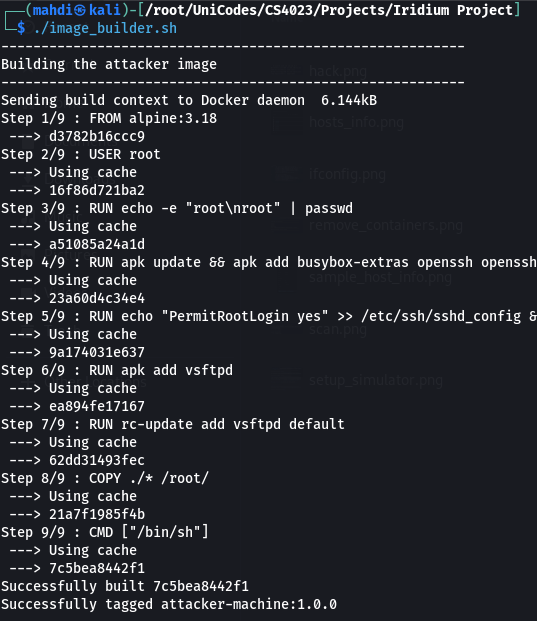
\includegraphics[width=0.5\linewidth]{images/image_builder.png}
    \caption{راه‌اندازی \lr{image}ها}
    \label{fig:image_builder}
\end{figure}

\begin{figure}[h!]
    \centering
    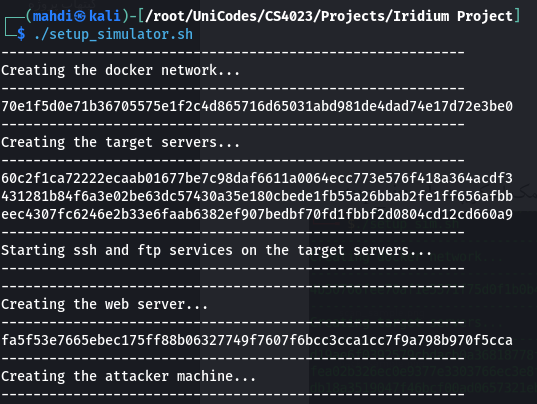
\includegraphics[width=0.5\linewidth]{images/setup_simulator.png}
    \caption{اجرای کانتینرها}
    \label{fig:setup_simulator}
\end{figure}


\section{حمله به سیستم‌های هدف}

ابتدا ادرس \lr{network} شبکه داکر که کانتینرها در آن در حال اجرا هستند را پیدا کرده و سپس با اجرای فایل \lr{scan.sh} نتایج مورد نظر در فایل \lr{openports.csv} ذخیره می‌شوند. سپس با اجرای \lr{hack.sh} حمله آغاز می‌شود و در هر دقیقه یک بار اطلاعات امنیتی سیستم های هدف در دیتابیس ذخیره می‌شوند.

\begin{figure}[h!]
    \centering
    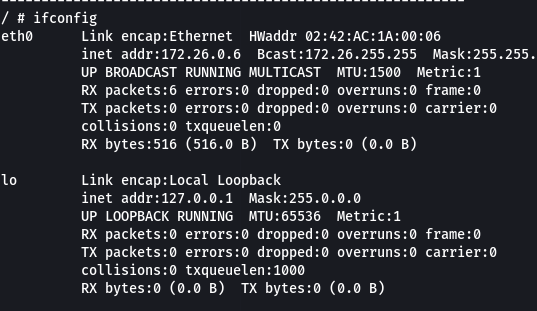
\includegraphics[width=0.5\linewidth]{images/ifconfig.png}
    \caption{اسکن‌کردن شبکه}
    \label{fig:ifconfig}
\end{figure}

\begin{figure}[h!]
    \centering
    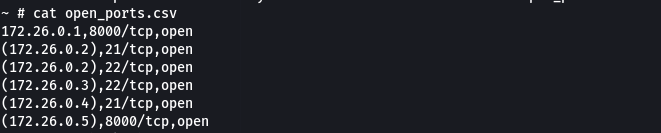
\includegraphics[width=0.5\linewidth]{images/open_ports.png}
    \caption{پورت‌های باز پیداشده}
    \label{fig:open_ports}
\end{figure}

\begin{figure}[h!]
    \centering
    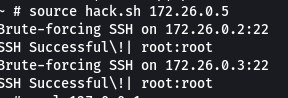
\includegraphics[width=0.5\linewidth]{images/hack.png}
    \caption{اجرای اسکریپت \lr{hack}}
    \label{fig:hack}
\end{figure}

\begin{figure}[h!]
    \centering
    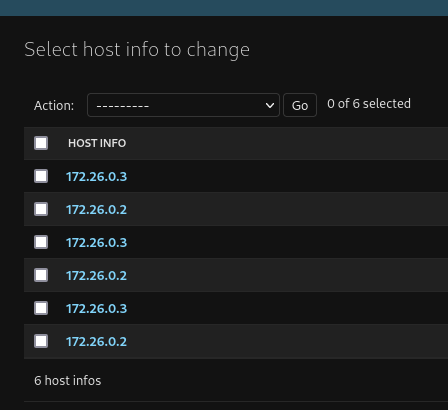
\includegraphics[width=0.5\linewidth]{images/hosts.png}
    \caption{هاست‌های ذخیره‌شده در دیتابیس}
    \label{fig:hosts}
\end{figure}


\section{پایان حمله}

در نهایت با استفاده از اسکریپت \lr{removecontainers.sh} کانتینرهای در حال اجرا را متوقف کرده و شبکه داکر را حذف می‌کنیم. 

\begin{figure}[h!]
    \centering
    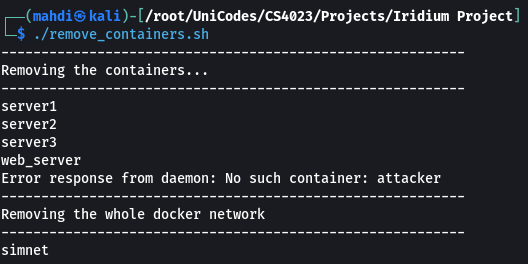
\includegraphics[width=0.5\linewidth]{images/remove_containers.png}
    \caption{حذف کانتینر‌ها و پایان حمله}
    \label{fig:remove_containers}
\end{figure}


\section{داکرهاب و گیت‌هاب}
\lr{Image} هریک از بخش‌های پروژه در \href{https://hub.docker.com/r/imahdighazavi/iridium-project/tags}{در این لینک} و کد پروژه پیاده‌شده \href{https://github.com/iMahdiGhazavi/iridium-project}{در این لینک} گیت‌هاب قرار دارند. 



